{\color{indiagreen}\subsection{Potencialna energija}}
\begin{center}
	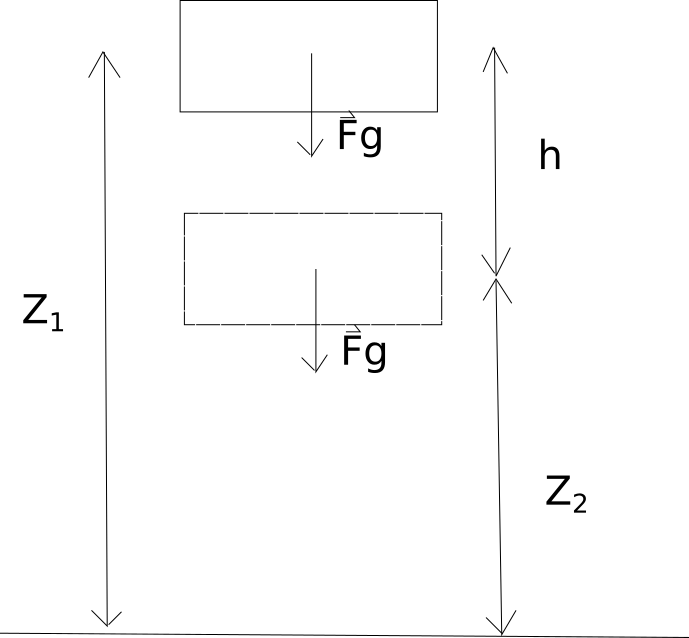
\includegraphics[width=15cm, height=15cm,keepaspectratio=true]{Potencialna_energija.png}
\end{center}
$A = A_t + A_o$\\
A \dots delo vseh zunanjih sil\\
$A_t$ \dots delo teže\\
$A_o$ \dots delo vseh zunanjih sil razen teže\\
\textbf{SPUŠČANJE TELESA}
\begin{center}
	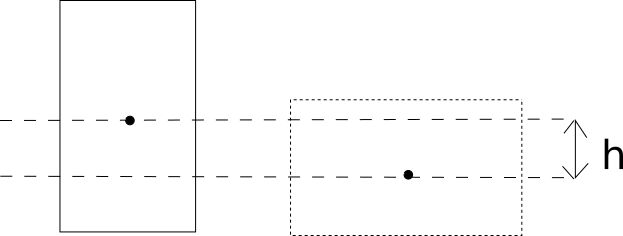
\includegraphics[width=15cm, height=15cm,keepaspectratio=true]{Potencialna_energija2.png}
\end{center}
\begin{align*}
	A_t &= Fs\\
	F &= F_g = mg\\
	s &= z_1 - z_2 \text{$z_1 \dots razdalja med prijemališčem sile in tlemi$}\\
	A_t &= mgz_1 - mgz_2\\
	{\color{bostonuniversityred}W_p} &= {\color{bostonuniversityred}mgz[j]} \text{\dots potencialna energija}\\
	A_t &= W_{p1} - W_{p2}\\
	{\color{bostonuniversityred}\Delta W_p} &= {\color{bostonuniversityred}mgh}\\
	{\color{bostonuniversityred}A_t} &= {\color{bostonuniversityred}\Delta W_p}\\
\end{align*}
\textbf{POSEBNI PRIMERI}
\begin{center}
	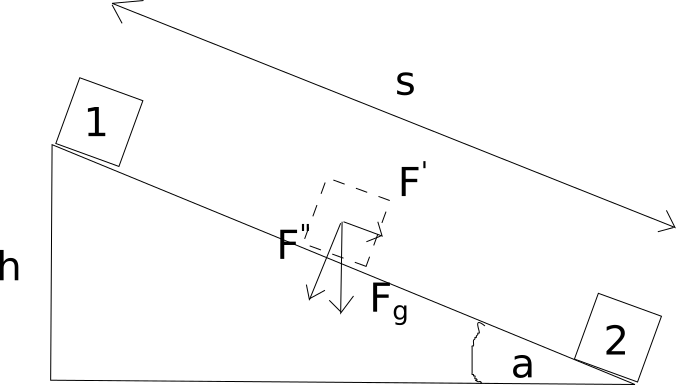
\includegraphics[width=15cm, height=15cm,keepaspectratio=true]{Potencialna_energija3.png}
\end{center}
\begin{align*}
	A &= F^{'}s\\
	F^{'} &= F_g \sin\varphi = mg\sin\varphi\\
	A &= mg\sin\varphi s\\
	\sin\varphi &= \frac{h}{s}\\
	A &= mg\frac{h}{\cancelto{}{s}} \cancelto{}{s}\\
	{\color{bostonuniversityred}A} &= {\color{bostonuniversityred}mgh} \text{//delo teže odvisno samo od višinske razlike}\\
\end{align*}
